\section{Workflow}
% Workflow teorico del processo
L'impostazione teorica del processo di digitalizzazione dell'informazione sonora contenuta nei dischi shellac si articola su quattro fasi principali:
\begin{itemize}
	\item scansione
	\item image processing
	\item sound extraction
	\item filtering
\end{itemize}
\begin{figure}[h!t]
\begin{center}
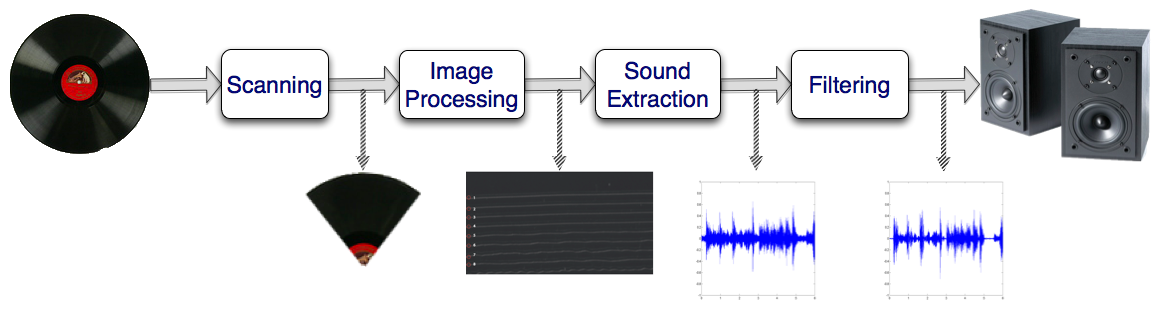
\includegraphics[scale=0.2]{./img/block-scheme.png}
\caption{Workflow generale}
\end{center}
\end{figure}

\subsection{Considerazioni preliminari}
Sono state messe in atto alcune considerazioni effettuate in fase 
preliminare, al fine di capire la fattibilità del progetto e per cercare
di evincere alcune specifiche; si è pensato che fosse fondamentale farsi
un'idea della correlazione, necessariamente presente, tra risoluzione
della scansione e qualità del segnale ottenuto, almeno nella fase precedente
al filtraggio. Si sono fatti, in particolare, alcuni test sulla base di
alcune semplici considerazioni: calcolando le dimensioni di un pixel, al
variare della risoluzione, e conoscendo le misure relative alle traccie
impresse sul disco, si è potuto ottenere il numero di pixel dedicati alla
traccia stessa. Il passo successivo è stato quello di simulare, usando
\textsc{Matlab} e alcuni brani musicali in qualità cd, il processo di 
acquisizione in funzione delle considerazioni fatte: si è attuato un 
processo di \emph{decimazione} del brano originale, cos\'i da ottenere una
stima della qualità ottenibile. \\
Queste prove hanno permesso di giungere alla conclusione che una risoluzione
di 2400 dpi potesse essere un buon compromesso tra qualità del suono e
trattabilità, computazionalmente parlando.

\subsection{Shellac}
I dischi in gommalacca, seppur soggetti a variazioni dovute ai diversi produttori e periodi di produzione, evidenziano delle caratteristiche il pi\`u delle volte comuni:
\begin{itemize}
	\item diametro tra gli 8 e 12 pollici
	\item massima escursione possibile del solco: 0.15 mm
	\item banda teorica: da 30 Hz 1.6 kHz
	\item banda reale: da 500 Hz a 3.5 kHz
\end{itemize}
Un primo problema che affligge il processo in questione pu\`o, anche intuitivamente, essere dedotto dall'osservazione della massima escursione possibile del solco: 0.15 mm, in poco pi\`u di un decimo di millimetro \`e infatti contenuta tutta l'informazione sonora che si vuole digitalizzare, di conseguenza la risoluzione dell'immagine ottenuta attraverso il processo di scansione dev'essere sufficientemente alta da poter recuperare il preciso andamento dei solchi.

\subsection{Scansione}
La fase di scansione permette di ottenere l'immagine delle tracce che verr\`a in seguito processata.
\begin{figure}[h!t]
\begin{center}
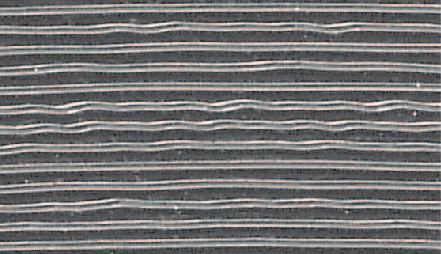
\includegraphics[scale=0.6]{./img/shellac-track.png}
\caption{Porzione di tracce}
\end{center}
\end{figure}
Ottenere un'immagine sufficientemente dettagliata da essere usata negli step successivi di elaborazione si \`e rivelata la fase pi\`u aleatoria dell'intero processo, il livello qualitativo \`e infatti inficiato da svariati fattori derivanti dallo scanner utilizzato e dal posizionamento del disco stesso sul piano del dispositivo.

Dai risultati sperimentali di questa fase \`e emersa la necessit\`a di utilizzare una risoluzione di scansione di 2400 dpi ottici (cio\`e non derivanti da interpolazione software operata dal driver dello scanner) e di rilevare - per ogni scanner utilizzato - il punto di illuminazione ottimale al fine di determinare la porzione di informazione contenente la maggior quantit\`a possibile di informazione.

Il punto di illuminazione ottimale \`e risultato ampiamente variabile a seconda del modello di scanner utilizzato determinando, di conseguenza, la necessit\`a di intraprendere un processo di calibrazione tutte le volte che risulti necessario cambiare dispositivo.

\subsection{Image processing}
La fase di image processing si articola in tre passaggi fondamentali:
\begin{itemize}
	\item ricerca del centro
	\item unwrap dell'immagine
	\item crop dell'immagine
\end{itemize}

\subsubsection{Ricerca del centro}
\begin{figure}[h!t]
\begin{center}
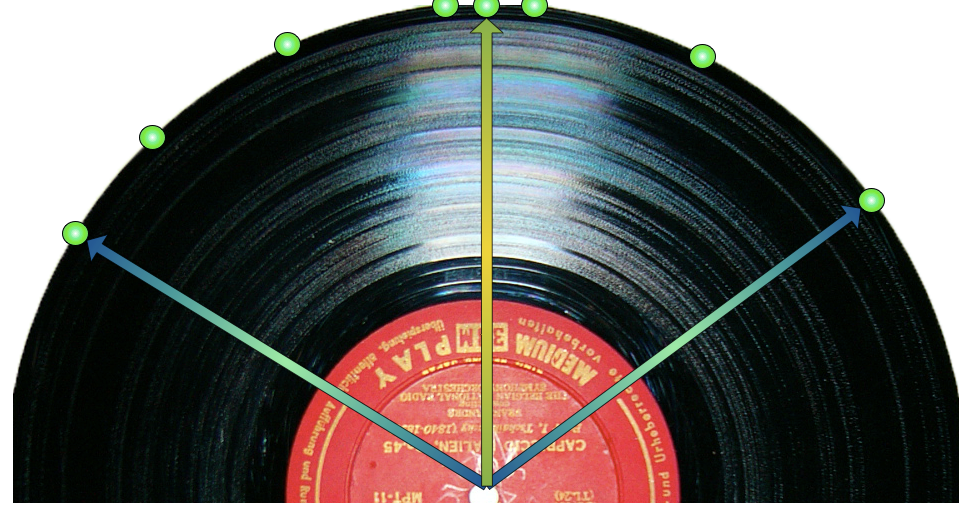
\includegraphics[scale=0.15]{./img/center.png}
\caption{Ricerca del centro}
\end{center}
\end{figure}
La determinazione del centro del disco scannerizzato \`e necessaria alla successiva trasformazione da coordinate cartesiane a coordinate polari che permette di ``raddrizzare'' le tracce.

La detection del centro ha inizio con la determinazione dei bordi del disco sulla base della variazione di luminosit\`a tra lo sfondo dell'immagine (bianco) e la porzione di disco acquisita tramite scansione (sensibilmente pi\`u scura).
Una volta acquisito un numero $N$ di coppie di punti $(x_i,y_i)$ giacenti sul bordo del disco, siano $(x_c, y_c)$ le coordinate del centro e $r$ il raggio del disco, si procede alla soluzione dell'equazione:
$$(x_i-x_c)^2+(y_i-y_c)^2=r^2 \quad i=1,2,\ldots,N$$
che pu\`o essere riscritta come:
$$r^2-x_c^2-y_c^2+2x_cx_i+2y_cy_i = x_i^2+y_i^2$$
e ponendo:
$$
\begin{cases}
a_1= r^2 - x_c^2 - y_c^2\\
a_2 = 2x_c\\
a_3 = 2y_c\\
\end{cases}
$$
si ottiene la forma matriciale:
$$
\begin{pmatrix}
1 && x_1 && y_1\\
1 && x_2 && y_2\\
\vdots && \vdots && \vdots\\
1 && x_N && y_N
\end{pmatrix}
\begin{pmatrix}
a_1 \\
a_2 \\
a_3
\end{pmatrix}
$$
$$
=
\begin{pmatrix}
x_1^2+y_1^2\\
x_2^2+y_2^2\\
\vdots \\
x_N^2+y_N^2
\end{pmatrix}
$$
che, risolta per mezzo del metodo di eliminazione di Gauss-Jordan, fornisce i parametri della circonferenza esterna del disco in esame:
$$
\begin{cases}
	x_c ={a_2\over{2}} \\
	y_c = {a_3\over{2}}\\
	r = \sqrt{x_c^2+y_c^2 + a_3}\\
\end{cases}
$$
\subsubsection{Unwrap}
Una volta determinato il centro del disco, si procede al ``raddrizzamento'' delle tracce per mezzo della trasformazione da coordinate cartesiane a polari:
\begin{figure}[h!t]
\begin{center}
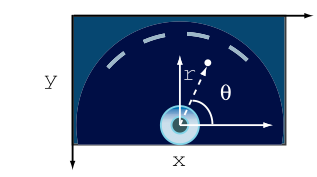
\includegraphics[scale=0.5]{./img/cartesio.png}
\caption{Rappresentazione in coordinate cartesiane}\label{cartesio}
\end{center}
\end{figure}

\begin{figure}[h!t]
\begin{center}
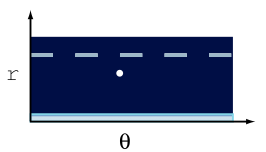
\includegraphics[scale=0.5]{./img/polare.png}
\caption{Rappresentazione in coordinate polari}
\end{center}
\end{figure}
Sia $v(x,y)$ un punto dell'immagine in coordinate cartesiane, la sua trasformazione in coordinate polari sar\`a: $u(r,\theta) = v(x_c+rcos(\theta), y_c+rsin(\theta))$, dove $r$ e $\theta$ sono definiti in figura \ref{cartesio}
\subsubsection{Crop}
Il cropping elimina parti non necessarie dell'immagine, come per esempio quelle relative all'etichetta, in modo da ottenere un file di
\begin{figure}[h!t]
\begin{center}
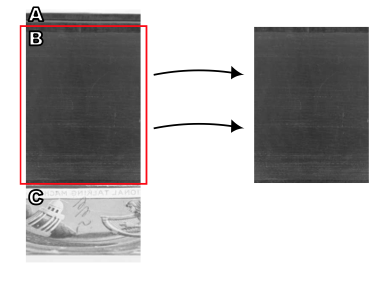
\includegraphics[scale=0.6]{./img/cropping.png}
\caption{Esempio di cropping}
\end{center}
\end{figure}
 dimensioni minori contenente solo l'informazione necessaria al processo.
\subsection{Sound extraction}

\subsubsection{Ricerca delle tracce}
Una volta determinato il centro e croppata l'immagine si prosegue alla localizzazione delle tracce ed al loro inseguimento.

Ogni immagine derivante da scansione viene memorizzata in forma matriciale 
$$I(h,w) = \begin{pmatrix} 
	I(1,1) && \ldots && I(1,w) \\
	\vdots && \vdots && \vdots \\
	I(h,1) && \ldots && I(h,w)
\end{pmatrix}$$  $$I(h,w) \in \{0, 1,2,\ldots, 255\}$$
L'algoritmo di localizzazione fa affidamento sul fatto che i pixel appartenenti a tracce risultino molto pi\`u luminosi rispetto agli altri, quindi sommando i pixel relativi alle righe di $I(h,w)$ (facendo quindi variare l'indice di colonna) si avranno dei picchi in corrispondenza delle tracce (righe).
\begin{figure}[h!t]
\begin{center}
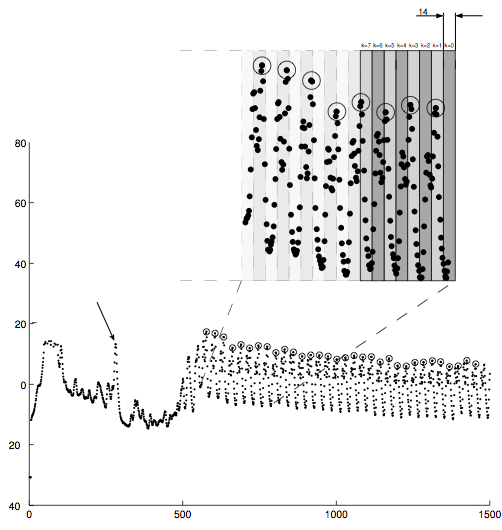
\includegraphics[scale=0.3]{./img/track-detection.png}
\caption{Picchi generati dall'algoritmo di localizzazione}
\end{center}
\end{figure}
\subsubsection{Inseguimeno delle tracce}
La conoscenza dei punti iniziali delle tracce nell'immagine scansionata permette il loro inseguimento per mezzo di un algoritmo euristico ad hoc.

Innanzitutto un vettore di 5 pixel di altezza viene centrato sul punto iniziale della traccia da seguire:
$$
P = 
\begin{pmatrix}
M(y_1+r(0), c)\\
\vdots \\
M(y+1+r(4), c)
\end{pmatrix}
$$
dove $r(i) \in \{-2,-1,0,1,2\}$ e c \`e l'indice di colonna.

Questi valori sono poi usati come pesi per il calcolo del centro di massa del vettore (corrispondente alla posizione della traccia relativamente alla colonna in cui quest'ultimo \`e stato posto): $\rho(n) = {\sum_{i=1}^{5}{P(i)r(i)}\over{\sum_{i=1}^{5}{P(i)c}}}$
\begin{figure}[h!t]
\begin{center}
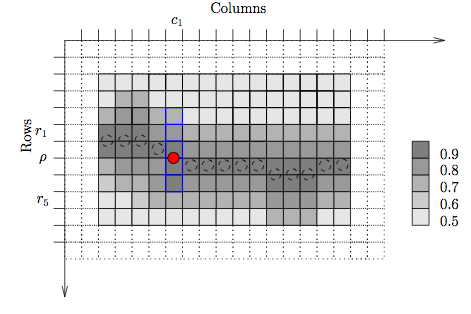
\includegraphics[scale=0.5]{./img/track-following.png}
\caption{Inseguimento delle tracce}
\end{center}
\end{figure}
Ad ogni passo dell'algoritmo il vettore di 5 pixel viene spostato in avanti di una colonna e ne viene determinato il centrodi massa.
\subsubsection{Concatenazione delle tracce}
\begin{figure}[h!t]
\begin{center}
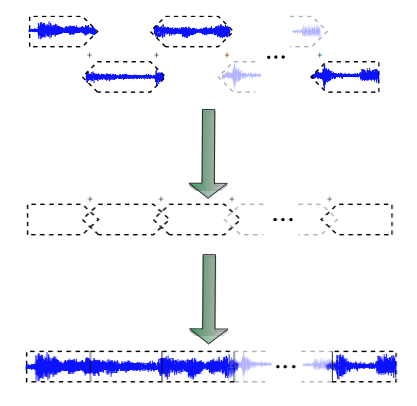
\includegraphics[scale=0.4]{./img/concatenation.png}
\caption{Concatenazione delle tracce}\label{fading}
\end{center}
\end{figure}
Una volta ottenuti gli spezzoni ti tracce da ogni singola immagine, questi devono essere concatenati in modo da ricostruire il brano originale. Una spiegazione grafica di questo processo \`e offerta in figura \ref{fading}
\section{Il progetto analizzato}
L'analisi del progetto sviluppato presso la Princeton University da Mark McCann, Paul Calamia e Nir Ailon si \`e articolata in quattro fasi:
\begin{itemize}
\item Analisi del codice Matlab
\item Creazione del flusso di lavoro
\item Associazione tra flusso del codice e modello teorico
\item Debugging e refactoring del codice
\end{itemize}

\subsection{Analisi del codice ed estrapolazione del flusso di lavoro}
La parte più rilevante, in termini di ore-uomo richieste, riguardo il
progetto è stata probabilmente quella relativa all'analisi e al refactoring
del codice sviluppato ma McCann et al. \\
Il processo di analisi ha posto le sue radici nella creazione di un 
workflow che descrivesse le dipendenze, logiche e temporali, delle chiamate
presenti nel codice[inserire ref]. 
\begin{figure}[h!t]
\begin{center}
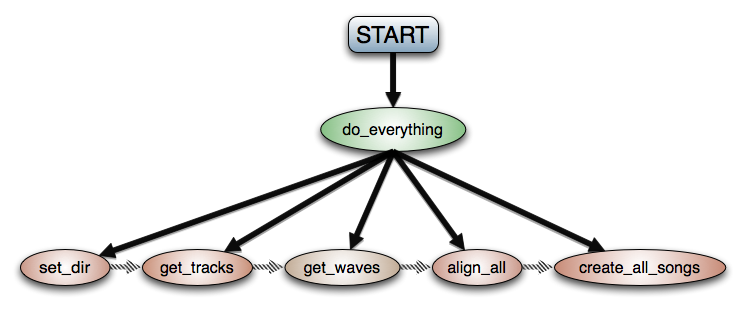
\includegraphics[scale=0.3]{./img/workflow.png}
\caption{Parte dell'albero che descrive il flusso del codice}\label{fading}
\end{center}
\end{figure}
Successivamente, si è cercato di capire 
se il codice fosse o meno funzionante e quali fossero i risultati 
ottenibili. \\
Il software presentava svariati errori logici piuttosto banali, che 
comunque compromettevano la produzione dell'output promesso. Partendo
dall'assunto che la procedura di correzione è stata talmente
onerosa che non è stato possibile indagare sulla corretta implementazione
dell'idea, si pone sotto una breve lista degli errori rilevati e una 
descrizione di massima di alcune caratteristiche strutturali del codice.

\begin{itemize}
\item Presenza, come già accennato, di errori logici relativamente banali. 
Per esempio in \texttt{get\_track.m} c'era un \texttt{Gnum\_scans} che era 
una stringa anzichè un numero, e andava valutata. (commit 331ba17a);
\item Non prevista la gestione di immagini non in scala di grigi;
\item Nella procedura di \emph{detection} dei bordi, la
\emph{threshold} era troppo alta (veniva fatta una spaccatura bianco-nero). 
Praticamente non veniva trovato il bordo a causa di una componente
grigia sullo sfondo delle nostre scansioni (commit 8b528741);
\item Qualora poi fosse presente dell'errore nel rilevamento del numero 
di traccie 
per scansione, il match falliva. Ad esempio, se la scansione nord 
dava 10 traccie e la scansione est ne dava 8 il software usciva in malo
modo. Una soluzione, seppur parziale, è stata quella di usare 
sempre l'ultima riga nel caso ne mancassero (commit 331ba17a).
\end{itemize}

Oltre a ciò può essere utile considerare che, in mezzo al codice, erano
presenti molte routine abbandonate o rimpiazzate e commentate: questo 
aspetto meriterebbe forse attenzione, in particolare, può essere utile
capire perché ci siano delle funzioni scritte ma non utilizzate.

Per meglio muoversi all'interno del codice, può infine essere d'aiuto
sapere che sono presenti delle subroutine che permettono di riprendere 
l'esecuzione, partendo da dati parziali.
